% Chapter 10

\chapter{Cross over and numerical analysis} % Main chapter title

\label{Chapter10} % For referencing the chapter elsewhere, use \ref{Chapter9} 

\lhead{Part III. \emph{Two wires}}
\chead{Chapter 10. \emph{Cross over \& numerical analysis}} % This is for the header on each page - perhaps a shortened title

%----------------------------------------------------------------------------------------
In this chapter we present the numerical analysis and results of the two wire system. The most noticeable of the results is, that we are able to find an interval of interwire distances, where both $s$- and $p$-wave type pairings exist, and that this is the energetically favourable state of the system.

\section{Cross over region and energy considerations}
\label{sec.2wiresCrossover_energy}
In this section we will show numerically, that during the transition from interwire to intrawire pairing the energetically favourable state of the system is the one where the interwire pairing is purely imaginary. We will further show, that this transition is characterized by having both the interwire and intrawire pairing simultaneously nonzero over an interval of interwire distances, $d$. 

We first come with an energy analysis as described after equation \eqref{eq.2wiresGrandGroundStateEnergy}. Let us first calculate the free energy, when the two wires are just free fermion gases. For $T = 0$ the free energy is simply the sum of the kinetic energy $\frac{k^2}{2m_F}$ for $|k| < k_F$: 
\begin{equation}
F = 2\sum_{k, |k| < k_F} \frac{k^2}{2m_F} = \frac{\mathcal{L}}{\pi} \int^{k_F}_{-k_F} dk \frac{k^2}{2m_F} = \epsilon_{F,0} N_F \int^{1}_{-1} d\tilde{k}\; \tilde{k}^2 = \frac{2}{3}\epsilon_{F,0} N_F. 
\end{equation}

Now the numerical analysis. Common for all the analyses we do the following. We start at low values of $d$. First, we come with an initial guess for the pairings and the chemical potential. Second, the pairings and chemical potentials are inserting in the gap equations \ref{eq.2wiresgapequations} and an updated version of the pairings is obtained. Third, this is inserted into the number equation \ref{eq.2wiresnumberequation}, which gives an updated version of the chemical potential. Finally, this is iterated until the pairings are not altered by more than $0.1$\textperthousand. For each step of $d$ we then return to the same initial guess for the pairings to avoid any hysteresis in the analysis. We then use equation \eqref{eq.2wiresGrandGroundStateEnergy} to calculate the grand energy, $E_0$, and in turn the Helmholtz free energy $E_0 + 2\mu N_F$.  

If we let $\Delta^{12}_k = 0$ and search for nonzero $\Delta^{11}_k$ we get the dashed curve in figure \ref{fig.2wiresE0ddepend} for the specified set of parameters. Hence, this describes the situation where we only have intrawire pairing. It is independent of $d$ as it should be. Conversely, we can let $\Delta^{11}_k = 0 = \Delta^{22}_k$ and search for nonzero $\Delta^{12}_k$. This results in the dash-dotted curve. As we expect, these two curves intersect at some critical distance $d_c$. In the present case $k_Fd_c \approx 0.748$. The naively expected behaviour is then the following. For large distances, $d$, the intrawire pairing is energetically favourable and is therefore the only one present. As we decrease $d$ we get to the critical point $d_c$, where the interwire pairing becomes favourable in stead. For $d < d_c$ we would then expect the interwire pairing to be the only one present. This turns out to be the exact behaviour, if we force the interwire pairing to be real. The two types of pairings do not coexist, a sudden flip from one to the other occures. This is the blue curve in figure \ref{fig.2wiresE0ddepend}. 

The question now is: can we find a solution, where both pairings are present simultaneously and is this energetically favourable? The answer is the following. If we let $\Delta^{12}_k$ be purely imaginary and search for both nonzero $\Delta^{12}_k$ and $\Delta^{11}_k$, we get the red curve. This curve clearly represents the energetically favourable solution. Since the sudden flip between the two types of pairings is associated with the blue curve, the red curve must describe a coexistence of the two types of pairings. This we verify explicitly in the following analysis. 

For $\Delta^{12}_k$ real the analysis is performed in the same way as in the above. Only we record the pairings at the Fermi momentum: $\left|\Delta^{11}_{k_F}\right|$ and $\left|\Delta^{12}_{k_F}\right|$ as a function of $k_Fd$. This results in the blue curves in figure \ref{fig.2wiresMaximalPairingddepend}. The behaviour is largely as described above. When we increase $d$ the interwire pairing decreases, until we reach the critical distance $d_c$ where it suddenly flips to a intrawire pairing in stead. 

Now let us concentrate on the energetically favourable solution: $\Delta^{12}_k$ imaginary. In this case the energy dispersions are identical and even in $k$: $E^{\pm}_{F,k} = E_{F,k} = \sqrt{\varepsilon_k^2 + (\Delta^{11}_k)^2 + |\Delta^{12}_k|^2}$. This means, that the gap equations in \eqref{eq.2wiresgapequations} partially decouples: 
\begin{align}
\Delta^{11}_k &= -\frac{1}{\mathcal{L}}\sum_{k'} W_{\text{ind}}^{11}(k, k')\frac{\Delta^{11}_{k'}}{2E_{F,k'}}\tanh\left(\frac{\beta E_{F,k'}}{2}\right), \nonumber \\
\Delta^{12}_k &= -\frac{1}{\mathcal{L}}\sum_{k'} W_{\text{ind}}^{12}(k, k')\frac{\Delta^{12}_{k'}}{2E_{F,k'}}\tanh\left(\frac{\beta E_{F,k'}}{2}\right).
\label{eq.2wiresgapequationsDelta12imaginary}
\end{align} 
This explicitly shows, that the two pairings are only coupled through the energy $E_{F,k}$. We start the analysis around $d = d_c$, since both pairings are suspected to be present there. For each value of $d$ we do something very similar to the above. However, here we do not reinitiate the initial guess in each step of $d$. In stead we reuse the found solution from the previous value of $d$. This makes the analysis much faster, and as long as the transition between the pairings is continuous no mistake is made. Further, we record the pairings at the Fermi momentum as above. The result is shown as the red curves in figure \ref{fig.2wiresMaximalPairingddepend}.

\begin{figure} 
\begin{center}  
% GNUPLOT: LaTeX picture with Postscript
\begingroup
  \makeatletter
  \providecommand\color[2][]{%
    \GenericError{(gnuplot) \space\space\space\@spaces}{%
      Package color not loaded in conjunction with
      terminal option `colourtext'%
    }{See the gnuplot documentation for explanation.%
    }{Either use 'blacktext' in gnuplot or load the package
      color.sty in LaTeX.}%
    \renewcommand\color[2][]{}%
  }%
  \providecommand\includegraphics[2][]{%
    \GenericError{(gnuplot) \space\space\space\@spaces}{%
      Package graphicx or graphics not loaded%
    }{See the gnuplot documentation for explanation.%
    }{The gnuplot epslatex terminal needs graphicx.sty or graphics.sty.}%
    \renewcommand\includegraphics[2][]{}%
  }%
  \providecommand\rotatebox[2]{#2}%
  \@ifundefined{ifGPcolor}{%
    \newif\ifGPcolor
    \GPcolorfalse
  }{}%
  \@ifundefined{ifGPblacktext}{%
    \newif\ifGPblacktext
    \GPblacktexttrue
  }{}%
  % define a \g@addto@macro without @ in the name:
  \let\gplgaddtomacro\g@addto@macro
  % define empty templates for all commands taking text:
  \gdef\gplbacktext{}%
  \gdef\gplfronttext{}%
  \makeatother
  \ifGPblacktext
    % no textcolor at all
    \def\colorrgb#1{}%
    \def\colorgray#1{}%
  \else
    % gray or color?
    \ifGPcolor
      \def\colorrgb#1{\color[rgb]{#1}}%
      \def\colorgray#1{\color[gray]{#1}}%
      \expandafter\def\csname LTw\endcsname{\color{white}}%
      \expandafter\def\csname LTb\endcsname{\color{black}}%
      \expandafter\def\csname LTa\endcsname{\color{black}}%
      \expandafter\def\csname LT0\endcsname{\color[rgb]{1,0,0}}%
      \expandafter\def\csname LT1\endcsname{\color[rgb]{0,1,0}}%
      \expandafter\def\csname LT2\endcsname{\color[rgb]{0,0,1}}%
      \expandafter\def\csname LT3\endcsname{\color[rgb]{1,0,1}}%
      \expandafter\def\csname LT4\endcsname{\color[rgb]{0,1,1}}%
      \expandafter\def\csname LT5\endcsname{\color[rgb]{1,1,0}}%
      \expandafter\def\csname LT6\endcsname{\color[rgb]{0,0,0}}%
      \expandafter\def\csname LT7\endcsname{\color[rgb]{1,0.3,0}}%
      \expandafter\def\csname LT8\endcsname{\color[rgb]{0.5,0.5,0.5}}%
    \else
      % gray
      \def\colorrgb#1{\color{black}}%
      \def\colorgray#1{\color[gray]{#1}}%
      \expandafter\def\csname LTw\endcsname{\color{white}}%
      \expandafter\def\csname LTb\endcsname{\color{black}}%
      \expandafter\def\csname LTa\endcsname{\color{black}}%
      \expandafter\def\csname LT0\endcsname{\color{black}}%
      \expandafter\def\csname LT1\endcsname{\color{black}}%
      \expandafter\def\csname LT2\endcsname{\color{black}}%
      \expandafter\def\csname LT3\endcsname{\color{black}}%
      \expandafter\def\csname LT4\endcsname{\color{black}}%
      \expandafter\def\csname LT5\endcsname{\color{black}}%
      \expandafter\def\csname LT6\endcsname{\color{black}}%
      \expandafter\def\csname LT7\endcsname{\color{black}}%
      \expandafter\def\csname LT8\endcsname{\color{black}}%
    \fi
  \fi
    \setlength{\unitlength}{0.0500bp}%
    \ifx\gptboxheight\undefined%
      \newlength{\gptboxheight}%
      \newlength{\gptboxwidth}%
      \newsavebox{\gptboxtext}%
    \fi%
    \setlength{\fboxrule}{0.5pt}%
    \setlength{\fboxsep}{1pt}%
\begin{picture}(7200.00,5040.00)%
    \gplgaddtomacro\gplbacktext{%
      \csname LTb\endcsname%
      \put(946,767){\makebox(0,0)[r]{\strut{}$0.61$}}%
      \csname LTb\endcsname%
      \put(946,1293){\makebox(0,0)[r]{\strut{}$0.62$}}%
      \csname LTb\endcsname%
      \put(946,1819){\makebox(0,0)[r]{\strut{}$0.63$}}%
      \csname LTb\endcsname%
      \put(946,2345){\makebox(0,0)[r]{\strut{}$0.64$}}%
      \csname LTb\endcsname%
      \put(946,2872){\makebox(0,0)[r]{\strut{}$0.65$}}%
      \csname LTb\endcsname%
      \put(946,3398){\makebox(0,0)[r]{\strut{}$0.66$}}%
      \csname LTb\endcsname%
      \put(946,3924){\makebox(0,0)[r]{\strut{}$0.67$}}%
      \csname LTb\endcsname%
      \put(946,4450){\makebox(0,0)[r]{\strut{}$0.68$}}%
      \csname LTb\endcsname%
      \put(946,4976){\makebox(0,0)[r]{\strut{}$0.69$}}%
      \csname LTb\endcsname%
      \put(1141,484){\makebox(0,0){\strut{}$0.74$}}%
      \csname LTb\endcsname%
      \put(2261,484){\makebox(0,0){\strut{}$0.742$}}%
      \csname LTb\endcsname%
      \put(3381,484){\makebox(0,0){\strut{}$0.744$}}%
      \csname LTb\endcsname%
      \put(4500,484){\makebox(0,0){\strut{}$0.746$}}%
      \csname LTb\endcsname%
      \put(5620,484){\makebox(0,0){\strut{}$0.748$}}%
      \csname LTb\endcsname%
      \put(6740,484){\makebox(0,0){\strut{}$0.75$}}%
    }%
    \gplgaddtomacro\gplfronttext{%
      \csname LTb\endcsname%
      \put(176,2871){\rotatebox{-270}{\makebox(0,0){\strut{}$(E_0 + mu N_F)/(arepsilon_{F,0} N_F)$}}}%
      \put(3940,154){\makebox(0,0){\strut{}$k_Fd$}}%
      \csname LTb\endcsname%
      \put(5753,4803){\makebox(0,0)[r]{\strut{}$Interwire pairing real$}}%
    }%
    \gplbacktext
    \put(0,0){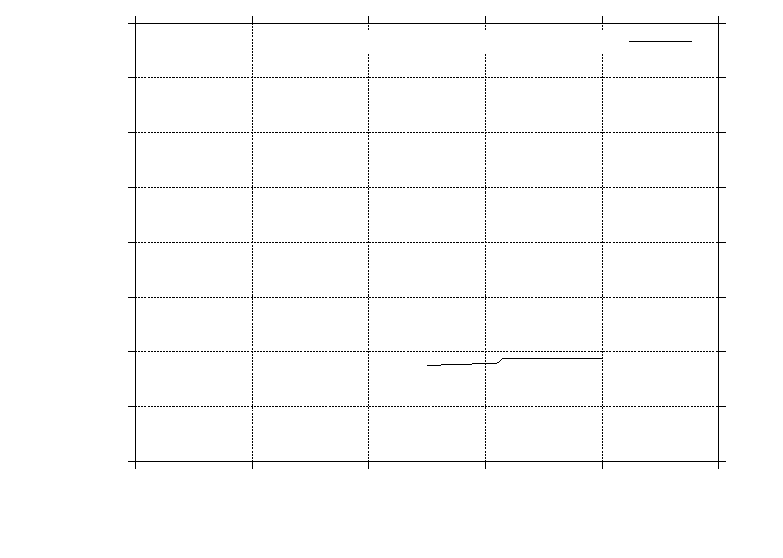
\includegraphics{E0ddepend}}%
    \gplfronttext
  \end{picture}%
\endgroup
  
\caption{The ground state free energy for $T = 0$, $E_0 + 2\mu N_F$, is plotted as a function of the interwire distance $d$. Black dashed: intrawire pairing only. Black dash-dotted: interwire pairing only. In red: $\Delta^{12}_k$ imaginary. In blue: $\Delta^{12}_k$ real. For the free gas: $(E_0 + 2\mu N_F)/\epsilon_{F,0}N_F = 2/3 = 0.667$. Parameters: $(n_Ba_B^3)^{1/3} = 0.01$, $(n_Ba_{BF}^3)^{1/3} = 0.11$, $l_t = 0$, $\frac{m_B}{m_F} = 7/40$, $\frac{n_F}{n_B^{1/3}} = 0.215$, $v_F/c_0 = 0.33$. }  
\label{fig.2wiresE0ddepend}  
\end{center}
\end{figure}

\begin{figure} 
\begin{center}  
% GNUPLOT: LaTeX picture with Postscript
\begingroup
  \makeatletter
  \providecommand\color[2][]{%
    \GenericError{(gnuplot) \space\space\space\@spaces}{%
      Package color not loaded in conjunction with
      terminal option `colourtext'%
    }{See the gnuplot documentation for explanation.%
    }{Either use 'blacktext' in gnuplot or load the package
      color.sty in LaTeX.}%
    \renewcommand\color[2][]{}%
  }%
  \providecommand\includegraphics[2][]{%
    \GenericError{(gnuplot) \space\space\space\@spaces}{%
      Package graphicx or graphics not loaded%
    }{See the gnuplot documentation for explanation.%
    }{The gnuplot epslatex terminal needs graphicx.sty or graphics.sty.}%
    \renewcommand\includegraphics[2][]{}%
  }%
  \providecommand\rotatebox[2]{#2}%
  \@ifundefined{ifGPcolor}{%
    \newif\ifGPcolor
    \GPcolorfalse
  }{}%
  \@ifundefined{ifGPblacktext}{%
    \newif\ifGPblacktext
    \GPblacktexttrue
  }{}%
  % define a \g@addto@macro without @ in the name:
  \let\gplgaddtomacro\g@addto@macro
  % define empty templates for all commands taking text:
  \gdef\gplbacktext{}%
  \gdef\gplfronttext{}%
  \makeatother
  \ifGPblacktext
    % no textcolor at all
    \def\colorrgb#1{}%
    \def\colorgray#1{}%
  \else
    % gray or color?
    \ifGPcolor
      \def\colorrgb#1{\color[rgb]{#1}}%
      \def\colorgray#1{\color[gray]{#1}}%
      \expandafter\def\csname LTw\endcsname{\color{white}}%
      \expandafter\def\csname LTb\endcsname{\color{black}}%
      \expandafter\def\csname LTa\endcsname{\color{black}}%
      \expandafter\def\csname LT0\endcsname{\color[rgb]{1,0,0}}%
      \expandafter\def\csname LT1\endcsname{\color[rgb]{0,1,0}}%
      \expandafter\def\csname LT2\endcsname{\color[rgb]{0,0,1}}%
      \expandafter\def\csname LT3\endcsname{\color[rgb]{1,0,1}}%
      \expandafter\def\csname LT4\endcsname{\color[rgb]{0,1,1}}%
      \expandafter\def\csname LT5\endcsname{\color[rgb]{1,1,0}}%
      \expandafter\def\csname LT6\endcsname{\color[rgb]{0,0,0}}%
      \expandafter\def\csname LT7\endcsname{\color[rgb]{1,0.3,0}}%
      \expandafter\def\csname LT8\endcsname{\color[rgb]{0.5,0.5,0.5}}%
    \else
      % gray
      \def\colorrgb#1{\color{black}}%
      \def\colorgray#1{\color[gray]{#1}}%
      \expandafter\def\csname LTw\endcsname{\color{white}}%
      \expandafter\def\csname LTb\endcsname{\color{black}}%
      \expandafter\def\csname LTa\endcsname{\color{black}}%
      \expandafter\def\csname LT0\endcsname{\color{black}}%
      \expandafter\def\csname LT1\endcsname{\color{black}}%
      \expandafter\def\csname LT2\endcsname{\color{black}}%
      \expandafter\def\csname LT3\endcsname{\color{black}}%
      \expandafter\def\csname LT4\endcsname{\color{black}}%
      \expandafter\def\csname LT5\endcsname{\color{black}}%
      \expandafter\def\csname LT6\endcsname{\color{black}}%
      \expandafter\def\csname LT7\endcsname{\color{black}}%
      \expandafter\def\csname LT8\endcsname{\color{black}}%
    \fi
  \fi
    \setlength{\unitlength}{0.0500bp}%
    \ifx\gptboxheight\undefined%
      \newlength{\gptboxheight}%
      \newlength{\gptboxwidth}%
      \newsavebox{\gptboxtext}%
    \fi%
    \setlength{\fboxrule}{0.5pt}%
    \setlength{\fboxsep}{1pt}%
\begin{picture}(7200.00,5040.00)%
    \gplgaddtomacro\gplbacktext{%
      \csname LTb\endcsname%
      \put(814,767){\makebox(0,0)[r]{\strut{}$0$}}%
      \csname LTb\endcsname%
      \put(814,1469){\makebox(0,0)[r]{\strut{}$0.1$}}%
      \csname LTb\endcsname%
      \put(814,2170){\makebox(0,0)[r]{\strut{}$0.2$}}%
      \csname LTb\endcsname%
      \put(814,2872){\makebox(0,0)[r]{\strut{}$0.3$}}%
      \csname LTb\endcsname%
      \put(814,3573){\makebox(0,0)[r]{\strut{}$0.4$}}%
      \csname LTb\endcsname%
      \put(814,4275){\makebox(0,0)[r]{\strut{}$0.5$}}%
      \csname LTb\endcsname%
      \put(814,4976){\makebox(0,0)[r]{\strut{}$0.6$}}%
      \csname LTb\endcsname%
      \put(1009,484){\makebox(0,0){\strut{}$0.71$}}%
      \csname LTb\endcsname%
      \put(1828,484){\makebox(0,0){\strut{}$0.72$}}%
      \csname LTb\endcsname%
      \put(2646,484){\makebox(0,0){\strut{}$0.73$}}%
      \csname LTb\endcsname%
      \put(3465,484){\makebox(0,0){\strut{}$0.74$}}%
      \csname LTb\endcsname%
      \put(4284,484){\makebox(0,0){\strut{}$0.75$}}%
      \csname LTb\endcsname%
      \put(5103,484){\makebox(0,0){\strut{}$0.76$}}%
      \csname LTb\endcsname%
      \put(5921,484){\makebox(0,0){\strut{}$0.77$}}%
      \csname LTb\endcsname%
      \put(6740,484){\makebox(0,0){\strut{}$0.78$}}%
    }%
    \gplgaddtomacro\gplfronttext{%
      \csname LTb\endcsname%
      \put(176,2871){\rotatebox{-270}{\makebox(0,0){\strut{}$Delta_k/epsilon_{F,0}$}}}%
      \put(3874,154){\makebox(0,0){\strut{}$k_Fd$}}%
      \csname LTb\endcsname%
      \put(3385,4803){\makebox(0,0)[r]{\strut{}$Intrawire pairing$}}%
      \csname LTb\endcsname%
      \put(3385,4583){\makebox(0,0)[r]{\strut{}$Interwire pairing$}}%
    }%
    \gplbacktext
    \put(0,0){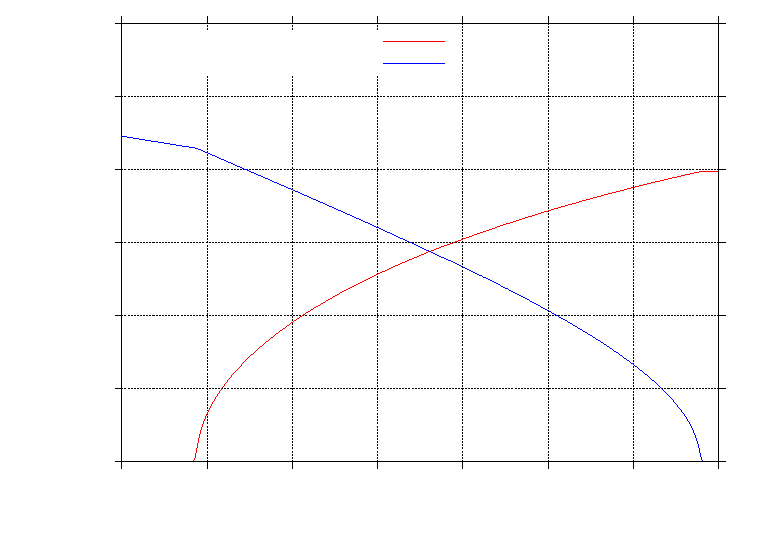
\includegraphics{ddepend}}%
    \gplfronttext
  \end{picture}%
\endgroup
  
\caption{The pairings at the Fermi momentum, $\left|\Delta^{11}_{k_F}\right|$ and $\left|\Delta^{12}_{k_F}\right|$, as a function of the distance $d$ between the wires. In red: pairings for $\Delta^{12}_k$ imaginary, corresponding to the red graph in figure \ref{fig.2wiresE0ddepend}. In blue: Pairings for $\Delta^{12}_k$ real, corresponding to the blue graph in figure \ref{fig.2wiresE0ddepend}. The \textit{inter}wire pairing is shown with dash-dotted lines. The \textit{intra}wire pairings are shown in solid. Parameters: $(n_Ba_B^3)^{1/3} = 0.01$, $(n_Ba_{BF}^3)^{1/3} = 0.11$, $l_t = 0$, $\frac{m_B}{m_F} = 7/40$, $\frac{n_F}{n_B^{1/3}} = 0.215$, $v_F/c_0 = 0.33$. }  
\label{fig.2wiresMaximalPairingddepend}  
\end{center}    
\end{figure}
 
We see, that for small and large distances the expected behaviour is observed. Naively it seems to be the case, that the interwire pairing increases linearly for small $k_Fd$. However, an analysis to lower values of $d$ shows, that it diverges for $d \to 0$ as expected. In between we see a continuous cross over region, where both pairings are present. Further, we notice that the intrawire pairing is constant from just under $k_Fd = 0.78$ and upwards as we expected. The fact that we start at $k_Fd = k_Fd_c = 0.748$, and then iterate downwards and upwards from there is the reason for the very small indent in the data precisely at this value.

The figure only shows the maximal pairing $\max_k[|\Delta_k|]$. The same analysis also gives us, how the pairings functionally change as the distance $d$ is varied. This is summarized in figure \ref{fig.pairingkdependT0dvaried}. This explicitly shows, that the interwire pairing is even in $k$ and hence is a $s$-wave type pairing. We see, that it has its maximum value at $k=0$ as one might expect from the interwire induced interaction. Further, it shows no oscillatory behaviour, it simply decays exponentially for large values of $k$. The intrawire pairing is seen to have the same functional form as for the single wire, hence a $p$-wave type pairing. The overall behaviour of the pairings are seen to be independent of $d$. The interwire pairing is simply enhanced as $d$ decreases, vice versa for the intrawire pairing.  

\begin{figure} 
\begin{center}  
% GNUPLOT: LaTeX picture with Postscript
\begingroup
  \makeatletter
  \providecommand\color[2][]{%
    \GenericError{(gnuplot) \space\space\space\@spaces}{%
      Package color not loaded in conjunction with
      terminal option `colourtext'%
    }{See the gnuplot documentation for explanation.%
    }{Either use 'blacktext' in gnuplot or load the package
      color.sty in LaTeX.}%
    \renewcommand\color[2][]{}%
  }%
  \providecommand\includegraphics[2][]{%
    \GenericError{(gnuplot) \space\space\space\@spaces}{%
      Package graphicx or graphics not loaded%
    }{See the gnuplot documentation for explanation.%
    }{The gnuplot epslatex terminal needs graphicx.sty or graphics.sty.}%
    \renewcommand\includegraphics[2][]{}%
  }%
  \providecommand\rotatebox[2]{#2}%
  \@ifundefined{ifGPcolor}{%
    \newif\ifGPcolor
    \GPcolorfalse
  }{}%
  \@ifundefined{ifGPblacktext}{%
    \newif\ifGPblacktext
    \GPblacktexttrue
  }{}%
  % define a \g@addto@macro without @ in the name:
  \let\gplgaddtomacro\g@addto@macro
  % define empty templates for all commands taking text:
  \gdef\gplbacktext{}%
  \gdef\gplfronttext{}%
  \makeatother
  \ifGPblacktext
    % no textcolor at all
    \def\colorrgb#1{}%
    \def\colorgray#1{}%
  \else
    % gray or color?
    \ifGPcolor
      \def\colorrgb#1{\color[rgb]{#1}}%
      \def\colorgray#1{\color[gray]{#1}}%
      \expandafter\def\csname LTw\endcsname{\color{white}}%
      \expandafter\def\csname LTb\endcsname{\color{black}}%
      \expandafter\def\csname LTa\endcsname{\color{black}}%
      \expandafter\def\csname LT0\endcsname{\color[rgb]{1,0,0}}%
      \expandafter\def\csname LT1\endcsname{\color[rgb]{0,1,0}}%
      \expandafter\def\csname LT2\endcsname{\color[rgb]{0,0,1}}%
      \expandafter\def\csname LT3\endcsname{\color[rgb]{1,0,1}}%
      \expandafter\def\csname LT4\endcsname{\color[rgb]{0,1,1}}%
      \expandafter\def\csname LT5\endcsname{\color[rgb]{1,1,0}}%
      \expandafter\def\csname LT6\endcsname{\color[rgb]{0,0,0}}%
      \expandafter\def\csname LT7\endcsname{\color[rgb]{1,0.3,0}}%
      \expandafter\def\csname LT8\endcsname{\color[rgb]{0.5,0.5,0.5}}%
    \else
      % gray
      \def\colorrgb#1{\color{black}}%
      \def\colorgray#1{\color[gray]{#1}}%
      \expandafter\def\csname LTw\endcsname{\color{white}}%
      \expandafter\def\csname LTb\endcsname{\color{black}}%
      \expandafter\def\csname LTa\endcsname{\color{black}}%
      \expandafter\def\csname LT0\endcsname{\color{black}}%
      \expandafter\def\csname LT1\endcsname{\color{black}}%
      \expandafter\def\csname LT2\endcsname{\color{black}}%
      \expandafter\def\csname LT3\endcsname{\color{black}}%
      \expandafter\def\csname LT4\endcsname{\color{black}}%
      \expandafter\def\csname LT5\endcsname{\color{black}}%
      \expandafter\def\csname LT6\endcsname{\color{black}}%
      \expandafter\def\csname LT7\endcsname{\color{black}}%
      \expandafter\def\csname LT8\endcsname{\color{black}}%
    \fi
  \fi
    \setlength{\unitlength}{0.0500bp}%
    \ifx\gptboxheight\undefined%
      \newlength{\gptboxheight}%
      \newlength{\gptboxwidth}%
      \newsavebox{\gptboxtext}%
    \fi%
    \setlength{\fboxrule}{0.5pt}%
    \setlength{\fboxsep}{1pt}%
\begin{picture}(7200.00,5040.00)%
    \gplgaddtomacro\gplbacktext{%
      \csname LTb\endcsname%
      \put(946,767){\makebox(0,0)[r]{\strut{}$-0.6$}}%
      \csname LTb\endcsname%
      \put(946,1468){\makebox(0,0)[r]{\strut{}$-0.4$}}%
      \csname LTb\endcsname%
      \put(946,2170){\makebox(0,0)[r]{\strut{}$-0.2$}}%
      \csname LTb\endcsname%
      \put(946,2871){\makebox(0,0)[r]{\strut{}$0$}}%
      \csname LTb\endcsname%
      \put(946,3573){\makebox(0,0)[r]{\strut{}$0.2$}}%
      \csname LTb\endcsname%
      \put(946,4275){\makebox(0,0)[r]{\strut{}$0.4$}}%
      \csname LTb\endcsname%
      \put(946,4976){\makebox(0,0)[r]{\strut{}$0.6$}}%
      \csname LTb\endcsname%
      \put(1141,484){\makebox(0,0){\strut{}$-10$}}%
      \csname LTb\endcsname%
      \put(2541,484){\makebox(0,0){\strut{}$-5$}}%
      \csname LTb\endcsname%
      \put(3941,484){\makebox(0,0){\strut{}$0$}}%
      \csname LTb\endcsname%
      \put(5340,484){\makebox(0,0){\strut{}$5$}}%
      \csname LTb\endcsname%
      \put(6740,484){\makebox(0,0){\strut{}$10$}}%
    }%
    \gplgaddtomacro\gplfronttext{%
      \csname LTb\endcsname%
      \put(176,2871){\rotatebox{-270}{\makebox(0,0){\strut{}$\Delta_k/\epsilon_{F,0}$}}}%
      \put(3940,154){\makebox(0,0){\strut{}$k/k_F$}}%
      \csname LTb\endcsname%
      \put(5753,1820){\makebox(0,0)[r]{\strut{}$k_Fd = 0.575$}}%
      \csname LTb\endcsname%
      \put(5753,1600){\makebox(0,0)[r]{\strut{}$k_Fd = 0.585$}}%
      \csname LTb\endcsname%
      \put(5753,1380){\makebox(0,0)[r]{\strut{}$k_Fd = 0.595$}}%
      \csname LTb\endcsname%
      \put(5753,1160){\makebox(0,0)[r]{\strut{}$k_Fd = 0.610$}}%
      \csname LTb\endcsname%
      \put(5753,940){\makebox(0,0)[r]{\strut{}$k_Fd = 0.620$}}%
    }%
    \gplbacktext
    \put(0,0){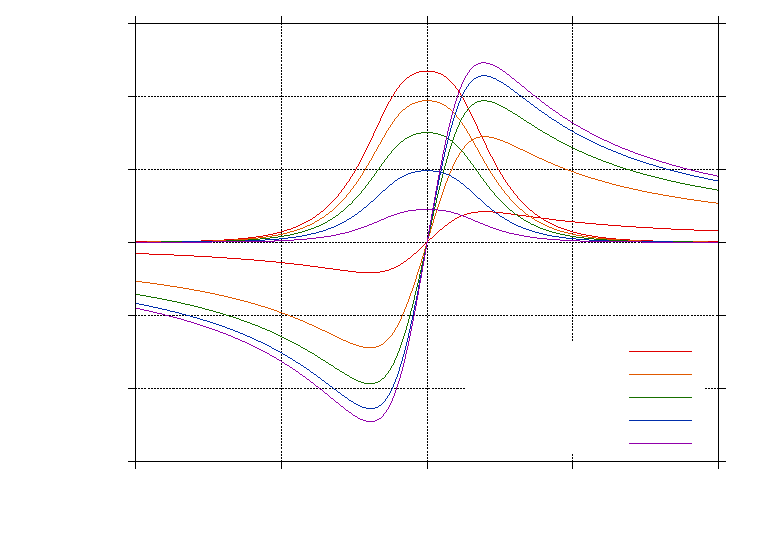
\includegraphics{Figures/twowires/Deltas1/kdepend}}%
    \gplfronttext
  \end{picture}%
\endgroup
  
\caption{The pairings $\Delta^{11}_k$ (odd) and $\Delta^{12}_k$ (even) plotted as a function of $k$ for $\Delta^{12}_k$ imaginary. We see, that the functional behaviour is independent of $d$, and that there is a cross over between interwire and intrawire dominated pairing. The intrawire pairing is increased as $d$ increases. Vice versa for the interwire pairing. Parameters: $(n_Ba_B^3)^{1/3} = 0.01$, $(n_Ba_{BF}^3)^{1/3} = 0.11$, $l_t = 0$, $\frac{m_B}{m_F} = 7/40$, $\frac{n_F}{n_B^{1/3}} = 0.215$, $v_F/c_0 = 0.33$. }  
\label{fig.pairingkdependT0dvaried}  
\end{center}    
\end{figure}

The combined result of the three figures tells us the following. We are able to find a cross over region of interwire distances $d$, where both an interwire $s$-wave pairing and an intrawire $p$-wave pairing is present, and this transition is the energetically favourable. 

\section{Edge states and the curious cross over}
\label{sec.2wiresedgestates_crossover_topology}
In this section we analyse the results of the previous section from a symmetry point of view. The analysis is based on the exact same ideas as in section \ref{sec.topindexandphases}. 

As pointed out in section \ref{sec.topindexandphases} the particle-hole symmetry ensures, that for every positive energy solution, there is also a negative one. For the separated wires sketched in the top of \ref{fig.2wiresedgestates} this has the same conclusion as in that section: there has to be a \textit{single} zero energy edge state which is robust against symmetry-conserving perturbations. The difference now is, that there are \textit{two} edge states: one for each wire. This has profound consequences. As we bring the wires closer together the system is perturbed by the interwire pairing $\Delta^{12}_k$. As shown in section \ref{sec.2wiressymmetries} this perturbation respects the particle-hole symmetry. This is simply because we are still dealing with a Bogoliubov de-Gennes system. 

\begin{figure}
\center
\begin{tikzpicture}
\draw[|->, thick] (0, 0) -- (0,  2) node[above]{$E$};
\draw[-, thick]   (0, 0) -- (0, -2);
\node at (-0.4, 0) {$0$};

\draw[-, dashed] (0, 1)--(2, 1);
\draw[-, thick] (-0.1, 1)--(0.1, 1);
\node at (-1.17,1) {$\min_k[E_{F,k}]$};

\draw[-, dashed] (0,    -1) -- (2,   -1);
\draw[-, thick]  (-0.1, -1) -- (0.1, -1);
\node at (-1.35,-1) {$-\min_k[E_{F,k}]$};

\draw[-, ultra thick] (1, 1)--(1, 2);
\draw[-, ultra thick] (1, -1)--(1, -2);
\node[red] at (1, 0) {\textbullet};

\draw[-, ultra thick] (2, 1)--(2, 2);
\draw[-, ultra thick] (2, -1)--(2, -2);
\node[blue] at (2, 0) {\textbullet};

\draw[-, dashed] (0,0.01) --(2,0.01);

\node at (3, -1.9) {$0$};
\node at (8, -1.9) {$\mathcal{L}$};
\draw[|->, thick ] (3,-1.5) -- (9,-1.5) node[right]{$x$};

\draw[-, ultra thick ] (3,-1.5) -- (8,-1.5);
\draw[scale=0.5,domain=-1:1,smooth,variable=\x,red] plot ({\x + 6},{ 3 * exp{- 10 * \x*\x} - 3});
\draw[scale=0.5,domain=-1:1,smooth,variable=\x,red] plot ({\x + 16},{ 3 * exp{- 10 * \x*\x} -3});

\node at (3, 1.1) {$0$};
\node at (8, 1.1) {$\mathcal{L}$};
\draw[|->, thick ] (3,1.5) -- (9,1.5) node[right]{$x$};

\draw[-, ultra thick] (3,1.5) -- (8,1.5);
\draw[scale=0.5,domain=-1:1,smooth,variable=\x,blue] plot ({\x + 6},{ 3 * exp{- 10 * \x*\x} + 3});
\draw[scale=0.5,domain=-1:1,smooth,variable=\x,blue] plot ({\x + 16},{ 3 * exp{- 10 * \x*\x} + 3});

\draw[-, dashed] (5.5, -1.5) -- (5.5, 1.5);
\node at (4.8, 0) {$d=\infty$};
\end{tikzpicture}

\begin{tikzpicture}
\draw[|->, thick] (0, 0) -- (0,  2) node[above]{$E$};
\draw[-, thick]   (0, 0) -- (0, -2);
\node at (-0.4, 0) {$0$};

\draw[-, dashed] (0, 1)--(2, 1);
\draw[-, thick] (-0.1, 1)--(0.1, 1);
\node at (-1.17,1) {$\min_k[E_{F,k}]$};

\draw[-, dashed] (0,    -1) -- (2,   -1);
\draw[-, thick]  (-0.1, -1) -- (0.1, -1);
\node at (-1.35,-1) {$-\min_k[E_{F,k}]$};

\draw[-, ultra thick] (1, 1)--(1, 2);
\draw[-, ultra thick] (1, -1)--(1, -2);
\node[red] at (1, 0) {\textbullet};
\draw[->] (1, 0) --  (1,  1);

\draw[-, ultra thick] (2, 1)--(2, 2);
\draw[-, ultra thick] (2, -1)--(2, -2);
\node[blue] at (2, 0) {\textbullet};
\draw[->] (2, 0) --  (2,  -1);

\draw[-, dashed] (0,0.01) --(2,0.01);

\node at (3, -1.9) {$0$};
\node at (8, -1.9) {$\mathcal{L}$};
\draw[|->, thick ] (3,-1.5) -- (9,-1.5) node[right]{$x$};

\draw[-, ultra thick ] (3,-1.5) -- (8,-1.5);

\node at (3, 1.1) {$0$};
\node at (8, 1.1) {$\mathcal{L}$};
\draw[|->, thick ] (3,1.5) -- (9,1.5) node[right]{$x$};

\draw[-, ultra thick] (3,1.5) -- (8,1.5);

\draw[-, dashed] (5.5, -1.5) -- (5.5, 1.5);
\node at (4.8, 0) {$d<\infty$};
\end{tikzpicture}
\caption{Top: for $d=\infty$ we have two copies of the single wire system. There are two symmetry-protected edge states, one at each wire. This is indicated with red and blue. Bottom: this is only for $\Delta^{12}_k$ imaginary. The interwire pairing respects the particle hole symmetry, but the edge states are no longer protected, since there are two of them. Consequently, there are no edge states.}
\label{fig.2wiresedgestates}
\end{figure}

Let us now first focus on the energetically favourable solution found in the previous section: $\Delta^{22}_k = - \Delta^{11}_k$ real and $\Delta^{12}_k$ imaginary. As shown in section \ref{sec.2wiressymmetries} this system has an additional time reversal symmetry that exhanges the wires, and that squares to $+\mathbb{I}$. However, there is nothing to protect the two edge states in the two wires from coupling, and since it is only the total spectrum that has to exhibit the plus/minus symmetry in the energies, the edge state energies can \textit{gap} away. This is sketched in the bottom of figure \ref{fig.2wiresedgestates}. This is exactly, what the numerical analysis says must be happening. The reason is the following. The separated wires exhibit only $p$-wave pairing, which has a topological ground state as shown in chapter \ref{Chapter7}. The closely spaced wires on the other hand have only $s$-wave pairing; a system that is known to be topologically trivial.\footnote{This we show explicitly in section \ref{sec.2wires_CSinv}.} Hence, according to the arguments of section \ref{sec.topindexandphases} either the bulk energy gap has to close, or the edge states are simply coupled and gapped away. In the case of an imaginary interwire pairing the energy dispersion is: $E_{F,k} = \sqrt{\varepsilon^2_k + (\Delta^{11}_k)^2 + |\Delta^{12}_k|^2 }$. This means, that the bulk energy gap \textit{cannot} close, since it only contains positive terms. The only possibility is, that $\varepsilon_k, \Delta^{11}_k$ and $\Delta^{12}_k$ are simultaneously zero. This is ruled out by the numerical analysis in figure \ref{fig.pairingkdependT0dvaried}. Since the bulk gap does not close, the edge states are gapped.

The situation changes dramatically for the real interwire pairing case. As shown in section \ref{sec.2wiressymmetries} this means, that the system has a time reversal symmetry, that squares to $-\mathbb{I}$. The edge states are hereby protected by Kramers degeneracy. The argument closely follows the argument in \cite{BernevigTITSC}. The time reversal symmetry in first quantization is in general described by an antiunitary operator $UK$, where $U$ is unitary, and $K$ is the complex conjugation operator. For the system at hand, we have: $\mathcal{T} = i\sigma_2 K$. Explicitly the symmetry looks like: $\mathcal{T}\mathcal{H}_{FF,k} = \mathcal{H}_{FF,-k}\mathcal{T}$. Let us now assume, that we have one state, $\ket{\psi_k}$, with energy $E_k$. Then $\mathcal{T}\ket{\psi_k}$ also has the energy $E_k$:
\begin{equation}
\mathcal{H}_{FF,-k}\mathcal{T}\ket{\psi_k} = \mathcal{T}\mathcal{H}_{FF,k}\ket{\psi_k} = E_k\mathcal{T}\ket{\psi_k}. \nonumber
\end{equation}
The above further shows, that the time reversed state is a state in $-k$, since it is an eigenstate to $\mathcal{H}_{FF,-k}$. Now we wish to show, that $\ket{\psi_k}$ and $\mathcal{T}\ket{\psi_k}$ are orthogonal. For this reason we note, that for any antiunitary operator we have the identity \cite{Sakurai, BernevigTITSC}:
\begin{equation}
\braket{\tilde{\psi}_1| \tilde{\psi}_2} = \braket{\psi_2|\psi_1}, \nonumber
\end{equation} 
where $\ket{\psi_j}$ are arbitrary states and $\ket{\tilde{\psi}_j} = T\ket{\psi_j}$. Hence, if we reverse the order of the states in the inner product, we get the inner product of the time reversed states. Now let $\ket{\tilde{\psi}_{-k}} = T\ket{\psi_k}$. Since $T^2 = - \mathbb{I}$ we have: $\ket{\psi_k} = -T^2\ket{\psi_k}= -T\ket{\tilde{\psi}_{-k}}$. With these relations we get:
\begin{equation}
\braket{\psi_k|\tilde{\psi}_{-k}} = -\braket{\psi_k|\tilde{\psi}_{-k}} \Rightarrow \braket{\psi_k|\tilde{\psi}_{-k}} = 0. 
\end{equation}
So the states are orthogonal. This tells us that for each energy $E_k$ there are at least two states, albeit possible at different $k$. This is the momentum space description of Kramers degeneracy. Notice, that it is crucial that $\mathcal{T}^2 = -\mathbb{I}$. For $\mathcal{T}^2 = +\mathbb{I}$ there is no Kramers degeneracy. 

The question now is, how this changes the behaviour from the imaginary interwire pairing case, if we only look at perturbations, that respect all the symmetries of the system. Before the edge states could gap away: one to positive and one to negative energies. However, that is not possible here, because it would lead to only a single state at those two energies. Hence, the edge states are once again protected at $E = 0$. Since we now know, that we have to come from a topological to a trivial state something dramatic must happen in the cross over. In the same way as in section \ref{sec.topindexandphases} the switch in topological to trivial phase is associated with a closing in the bulk energy gap. The numerical analysis shows, that this happens at a single point $d = d_c$. The curious issue is, that if we look at the dispersion relations nothing stops this transition from being continuous:
\begin{equation}
E^{\pm}_{F,k} = \sqrt{\varepsilon^2_k + (\Delta^{11}_k)^2 + (\Delta^{12}_k)^2 \pm 2\Delta^{11}_k\Delta^{12}_k} = \sqrt{\varepsilon^2_k + (\Delta^{11}_k \pm \Delta^{12}_k)^2}. \nonumber
\end{equation}
From this it is clear, that if we had both pairings nonzero over an interval of $d$, then for some distance $d$, we would have $\Delta^{11}_{\pm k} = \mp \Delta^{12}_k$ at the Fermi surface, where $\varepsilon_k = \frac{k^2}{2m_F} - \mu =  0$, hence leading to $E^{\pm}_{F,\pm k} = 0$. However, this does not happen. The transition is abrupt at a single point, $d = d_c$. Up till now this is therefore a curious numerical result. It is therefore part of the more thorough topological investigation of the next section.

\section{The Chern-Simons invariants}
\label{sec.2wires_CSinv}
In this section we will calculate the Chern-Simons topological invariant for the two wire system. In turn we will calculate the Wilson loop and use this to analyse the system topologically. 

The Berry connection for a system with several negative energy states becomes a matrix:
\begin{equation}
\mathcal{A}^{ij}_k = \bra{e^{-}_{i,k}}\partial_k\ket{e^{-}_{j,k}}.
\end{equation}
In the present case the Berry connection is a $2\times 2$ matrix. In the case of a $T^2 = + \mathbb{I}$ symmetry the topological invariant, $\nu$, is calculated in analogy to the one in section \ref{sec.CS1} and is given by the twice the Chern-Simons invariant:
\begin{align}
\nu &= 2\text{CS}_1 = \frac{i}{\pi} \int dk\; \text{tr}[\mathcal{A}] = \frac{i}{\pi} \int dk\; \left[\bra{e^{-}_{1,k}}\partial_k\ket{e^{-}_{1,k}} + \bra{e^{-}_{2,k}}\partial_k\ket{e^{-}_{2,k}}  \right] \nonumber \\
 &= 2(\text{CS}_{1,1} + \text{CS}_{1,2})\in \mathbb{Z}, \hspace{0.5cm} T^2 = +\mathbb{I}.
\label{eq.2wires.topinv.T2eqplus1}
\end{align}
Here we have indicated the contribution to the Chern-Simons invariant from the eigenvector $\ket{e^{-}_{i,k}}$ with $\text{CS}_{1,i}$. We will refer to these as the subsystem invariants. For $T^2 = +\mathbb{I}$ the subsystem invariants are not well-defined, only their sum is. For $T^2 = -1$ the Kramers degeneracy means, that as long as one Kramers partner is protected, so is the other. Since $\ket{e^{-}_{1,k}}$ and $\ket{e^{-}_{2,k}}$ are the only available eigenvectors to negative eigenvalues, these must be Kramers partners. Hence, the topological invariant is found by simply calculated either $\text{CS}_{1,1}$ or $\text{CS}_{1,2}$\cite{FuKane2006, LiYangChen}. Since in this case we are only searching for a $\mathbb{Z}_2$ invariant, we go to the Wilson loop:
\begin{equation}
\nu = W_{1,1} = \text{e}^{2\pi i\text{CS}_{1,1}} = \pm 1, \hspace{0.5cm} T^2 = -\mathbb{I}.
\label{eq.2wires.topinv.T2eqminus1}
\end{equation}
We are now ready for the computation. This will be done in the two cases $\Delta^{12}_k$ imaginary and real corresponding to the presence of a time reversal symmetry of the form $T^2 = +\mathbb{I}$ and $T^2 = -\mathbb{I}$ respectively. 

\subsection{$T^2 = +\mathbb{I}$, imaginary interwire pairing}
\label{subsec.2wires_CSinv_Delta12imag}
The aim of this subsection is to calculate $\nu$ as given in equation \eqref{eq.2wires.topinv.T2eqplus1}. We follow the same procedure as the one in section \ref{sec.CS1}. 

Since we differentiate the eigenvectors with respect to $k$, it is essential that these are well-behaved in any $k$. If we look closely at the eigenvectors derived back in section \ref{sec.2wiresgrandHFF}, we can see that if $\Delta^{12}_k = 0$, the eigenvectors are not well-behaved in $k = 0$. Back then this was no issue, since a single problem point in the integral makes no difference.\footnote{One might be concerned about this line of thinking. However, the gap equations in the special cases investigated in the current section have also been derived using well-behaved eigenvectors. The result is the same.} Hence, the single truly tricky part is to get well-behaved eigenvectors. However, there is a procedure for it, which was also used in section \ref{sec.CS1}. This procedure is described in \cite{Ryu.Topology}. First we transform the Hamiltonian to the standard Nambu spinor form, so that $C_k \to \tilde{C}_k = \begin{bmatrix} c_{1,k} & c_{2,k} & c^\dagger_{1,-k} & c^\dagger_{2,-k}  \end{bmatrix}$. This amounts to the following transformation of $\mathcal{H}_{FF,k}$:
\begin{align}
\mathcal{H}_{FF,k} &= \varepsilon_k \sigma_0 \otimes \tau_3 + \Delta^{11}_k \sigma_3 \otimes \tau_1 + \Delta^{12}_k \sigma_2 \otimes \tau_1 \to \nonumber \\
\mathcal{H}'_{FF,k} &= \varepsilon_k \sigma_3 \otimes \tau_0 + \Delta^{11}_k \sigma_1 \otimes \tau_3 + \Delta^{12}_k \sigma_1 \otimes \tau_2, \nonumber 
\end{align}
where $\otimes$ is the direct product, $\tau_i$ is the Pauli matrices in particle-hole space and $\sigma_i$ are the Pauli matrices in wire-space. We have also written the imaginary interwire pairing as $i\Delta^{12}_k$. Since the Hamiltonian belongs to symmetry class DIII it has a chiral symmetry: $\{S, \mathcal{H}_{FF,k}\} = 0$. In the new basis after the above transformation we see, that $S = \sigma_1\otimes \tau_1$. $S$ have eigenvectors $\ket{v_{ab}} = \ket{\chi^{1}_a}\otimes \ket{\chi^{1}_b}$, where $\ket{\chi^{1}_a}$ for $a = 1,2$ are the eigenvectors to the first Pauli matrix $\tau_1, \sigma_1$. We then transform to the basis, where $S$ is diagonal by forming $V = (\ket{v_{ab}})$ and calculating:
\begin{equation}
\tilde{\mathcal{H}}_{FF,k} = V^\dagger\mathcal{H}'_{FF,k}V = \varepsilon_k \sigma_1\otimes \tau_1 + \Delta^{11}_k \sigma_1\otimes\tau_3 - \Delta^{12}_k\sigma_2\otimes\tau_0. \nonumber 
\end{equation}
We then get the eigenvectors to negative energy eigenvalues:
\begin{equation}
\ket{e^{-}_{1,k}} = \frac{1}{\sqrt{2}E_{F,k}}\begin{bmatrix} \varepsilon_k \\ -\Delta^{11}_k + i\Delta^{12}_k \\ 0 \\ -E_{F,k} \end{bmatrix}, \hspace{0.5cm} \ket{e^{-}_{2,k}} = \frac{1}{\sqrt{2}E_{F,k}}\begin{bmatrix} \Delta^{11}_k + i\Delta^{12}_k \\ \varepsilon_k \\  -E_{F,k} \\ 0 \end{bmatrix},
\end{equation}
with $E_{F,k} = \sqrt{\varepsilon_k^2 + (\Delta^{11}_k)^2 + (\Delta^{12}_k)^2}$. These eigenvectors are manifestly well-defined for all $k$. Using these we explicitly get:
\begin{equation}
\mathcal{A}^{11}_k = \bra{e^{-}_{1,k}}\partial_k\ket{e^{-}_{1,k}} = -\frac{i}{2E_{F,k}^2}(\Delta^{11}_k\partial_k\Delta^{12}_k - \Delta^{12}_k\partial_k\Delta^{11}_k) = -\mathcal{A}^{22}_k. \nonumber
\end{equation}
Hereby: $\text{tr}[\mathcal{A}_k] = \mathcal{A}^{11}_k  + \mathcal{A}^{22}_k = 0$, and the topological invariant is simply $\nu = 0$. As for the single wire this is the topologically trivial value. This means, that the edge states formed in the single wire are not protected in the two wire system, when $T^2 = +\mathbb{I}$. This is consistent with the more pictorial analysis of the last section. 

\subsection{$T^2 = -\mathbb{I}$, real interwire pairing}
\label{subsec.2wires_CSinv_Delta12real}
In this subsection we calculate the topological invariant as defined in equation \eqref{eq.2wires.topinv.T2eqminus1}. 

To get to well-behaved eigenvectors we follow the same procedure as outlined in the previous subsection. The $\Delta^{12}_k$ of $\mathcal{H}_{FF,k}$ now has the form $\Delta^{12}_k \sigma_2 \otimes \tau_1$. After going to the Nambu spinor form, we therefore have $\mathcal{H}'_{FF,k} = \varepsilon_k \sigma_3 \otimes \tau_0 + \Delta^{11}_k \sigma_1 \otimes \tau_3 + \Delta^{12}_k \sigma_2 \otimes \tau_2$. The anticommuting symmetry is now given by: $S = \sigma_1\otimes \tau_2$. The corresponding eigenvectors are therefore $\ket{v_{ab}} = \ket{\chi^{1}_a}\otimes\ket{\chi^{2}_b}$. Letting $V = (\ket{v_{ab}})$ and calculating the conjugation of $\mathcal{H}'_{FF,k}$ then yields:
\begin{equation}
\tilde{\mathcal{H}}_{FF,k} = V^\dagger\mathcal{H}'_{FF,k}V = \varepsilon_k \sigma_1\otimes \tau_1 + \Delta^{11}_k \sigma_1\otimes\tau_3 - \Delta^{12}_k\sigma_2\otimes\tau_1. \nonumber 
\end{equation}
We only need a single negative energy eigenvector. We choose the one with eigenvalue $-E^+_{F,k} = -\sqrt{\varepsilon_k^2 + (\Delta^{11}_k + \Delta^{12}_k)^2}$: 
\begin{equation}
\ket{e^{-}_{1,k}} = \frac{1}{2E^{+}_{F,k}}\begin{bmatrix} \varepsilon_k + i(\Delta^{11}_k + \Delta^{12}_k) \\ i(\varepsilon_k + i(\Delta^{11}_k + \Delta^{12}_k)) \\ -iE^{+}_{F,k} \\ -E^{+}_{F,k} \end{bmatrix}. \nonumber
\end{equation}
This is seen to be manifestly well-defined for all $k$. The first element of the Berry connection is then:
\begin{equation}
\mathcal{A}^{11}_k = \bra{e^{-}_{1,k}}\partial_k\ket{e^{-}_{1,k}} = \frac{i}{2(E^{+}_{F,k})^2}\left(\varepsilon_k\partial_k(\Delta^{11}_k + \Delta^{12}_k) - (\Delta^{11}_k + \Delta^{12}_k)\partial_k \epsilon_k\right). \nonumber
\end{equation}
The subsystem Chern-Simons invariant hereby becomes: 
\begin{equation}
\text{CS}_{1,1} = \frac{1}{4\pi}\int dk \; \frac{\varepsilon_k\partial_k(\Delta^{11}_k + \Delta^{12}_k) - (\Delta^{11}_k + \Delta^{12}_k)\partial_k \epsilon_k}{\varepsilon_k^2 + (\Delta^{11}_k + \Delta^{12}_k)^2}. 
\label{eq.CS11integralform}
\end{equation}
We see, that this has the exact same structure has the single wire expression for $\text{CS}_{1}$, under the identification: $\Delta_k \to \Delta^{11}_k + \Delta^{12}_k$. The integrand therefore has a primitive in the same manner as in section \ref{sec.CS1}:
\begin{equation}
G_k(c) = -\arctan\left(\frac{\Delta^{11}_k + \Delta^{12}_k }{\varepsilon_k}\right) + c, \nonumber
\end{equation}
where $c$ is a constant. The evaluation of the integral itself however turns out to be a little subtle. Let us first take the simplest case: $\mu < 0$. For $\mu < 0$, $\varepsilon_k = \frac{k^2}{2m_F} - \mu$ is strictly positive for any $k$. This means, that $-\arctan\left(\frac{\Delta^{11}_k + \Delta^{12}_k }{\varepsilon_k}\right)$ is well-defined for all $k$ and we can use $G_k(c=0)$ as the primitive. Then:
\begin{equation}
\text{CS}_{1,1} = \frac{1}{4\pi}\left[-\arctan\left(\frac{\Delta^{11}_k + \Delta^{12}_k }{\varepsilon_k}\right)\right]^{\infty}_{-\infty} = 0, \nonumber
\end{equation}
as both $\Delta^{11}_k$ and $\Delta^{12}_k$ goes to $0$ and $\varepsilon_k \to \infty$ for $k\to \pm \infty$, and $\arctan(0) = 0$. Hence, for $\mu < 0$ we get $\nu = \text{e}^{2\pi i\text{CS}_{1,1}} = 1$ and the system is topologically trivial as for the single wire case. 

Now the more subtle $\mu > 0$ case. $\varepsilon_k$ has two zero points at the Fermi surface $k = \pm k_0$. This introduces discontinuities in $G_k(c=0)$ at $\pm k_0$. However, for the evaluation of the integral to be correct, we must use a continuous primitive. Therefore we have to patch a continuous solution together by looking in the intervals $k < k_-, k_- < k < k_+$ and $k>k_+$. Since $E_{F,k} \neq 0$ for all $k$ and $\varepsilon_{\pm k_0} = 0$, we get that $\Delta^{11}_{\pm k_0} + \Delta^{11}_{\pm k_0} \neq 0$. If this was not the case, the energy gap would close at either $+k_0$ or $-k_0$ and the topological index would be ill-defined. This means, that $\text{sgn}(\Delta^{11}_k + \Delta^{12}_k)$ is well-defined in $k = \pm k_0$. Hence, we get:
\begin{align}
\lim_{k \uparrow +k_0} G_k(c = 0)   &\overset{\varepsilon_k \uparrow 0}{=}   +\frac{\pi}{2}\text{sgn}(\Delta^{11}_{k_0} + \Delta^{12}_{k_0}), \nonumber \\
\lim_{k \downarrow +k_0} G_k(c = 0) &\overset{\varepsilon_k \downarrow 0}{=} -\frac{\pi}{2}\text{sgn}(\Delta^{11}_{k_0} + \Delta^{12}_{k_0}), \nonumber
\end{align}
since $\arctan(x) \to \pm \pi/2$ for $x \to \pm \infty$. To mend the discontinuity of $\pi\text{sgn}(\Delta^{11}_{k_+} + \Delta^{12}_{k_0})$, we let $c = \pi\text{sgn}(\Delta^{11}_{k_+} + \Delta^{12}_{k_0})$ for $k > k_0$. This was the $k > 0$ part. For $k \to -k_0$ we get analogously get:
\begin{align}
\lim_{k \downarrow -k_0} G_k(c = 0) &\overset{\varepsilon_k \uparrow 0}{=} +\frac{\pi}{2}\text{sgn}(-\Delta^{11}_{k_0} + \Delta^{12}_{k_0}), \nonumber \\
\lim_{k \uparrow -k_0} G_k(c = 0)   &\overset{\varepsilon_k \downarrow 0}{=} -\frac{\pi}{2}\text{sgn}(-\Delta^{11}_{k_0} + \Delta^{12}_{k_0}). \nonumber
\end{align}
Here we use, that $\Delta^{11}_k$ and $\Delta^{12}_k$ are respectively odd and even in $k$. We therefore let $c = \pi \text{sgn}(-\Delta^{11}_{k_0} + \Delta^{12}_{k_0})$ for $k < - k_0$. We have hereby constructed a continuous primitive to the integrand in equation \eqref{eq.CS11integralform}:
\begin{equation}
G_k = \left\{ \begin{matrix} 
-\arctan\left(\frac{\Delta^{11}_k + \Delta^{12}_k }{\varepsilon_k}\right) + \pi\text{sgn}(\Delta^{11}_{k_0} + \Delta^{12}_{k_0}), & k > k_0, \\
-\arctan\left(\frac{\Delta^{11}_k + \Delta^{12}_k }{\varepsilon_k}\right), & -k_0 \leq k \leq k_0, \\
-\arctan\left(\frac{\Delta^{11}_k + \Delta^{12}_k }{\varepsilon_k}\right) + \pi \text{sgn}(-\Delta^{11}_{k_0} + \Delta^{12}_{k_0}), & k < -k_0.
  \end{matrix} \right.
\label{eq.Gkmugreater0}
\end{equation}

Since the $\arctan$ part of $G_k$ goes to $0$ for $k\to \pm \infty$ we see, that the signs $\text{sgn}(\Delta^{11}_{\pm k_0} + \Delta^{12}_{\pm k_0})$ must be different for the integral to give a nonzero result. Since $\Delta^{12}_{k}$ is even and $\Delta^{11}_{k}$ is odd, this can only be achieved if $\Delta^{11}_{k}$ is dominant at the Fermi surface: $|\Delta^{11}_{k_0}| > |\Delta^{12}_{k_0}|$. Hence, we get:
\begin{equation}
\text{CS}_{1,1} = \frac{1}{4\pi} \left. G_k \right|^\infty_{-\infty} = \frac{1}{4}(\text{sgn}(\Delta^{11}_{k_0} + \Delta^{12}_{k_0}) - \text{sgn}(-\Delta^{11}_{k_0} + \Delta^{12}_{k_0})) = \left\{ \begin{matrix} 
\frac{1}{2}\text{sgn}(\Delta^{11}_{k_0} + \Delta^{12}_{k_0}) , & |\Delta^{11}_{k_0}| > |\Delta^{12}_{k_0}|, \\
0, & |\Delta^{11}_{k_0}| < |\Delta^{12}_{k_0}|.
  \end{matrix} \right. \nonumber 
\end{equation}

Finally, we can summarize the above calculations to the invariant:
\begin{equation}
\nu = \text{e}^{2\pi i \text{CS}_{1,1}} = \left\{ \begin{matrix} 
-1, & |\Delta^{11}_{k_0}| > |\Delta^{12}_{k_0}| & \text{and} & \mu > 0, \\
+1, & |\Delta^{11}_{k_0}| < |\Delta^{12}_{k_0}| & \text{or}  & \mu < 0.
  \end{matrix} \right.
\label{eq.CS11T2eqminus1}
\end{equation}
Hence, to be in a topological nontrivial phase we need $\mu > 0$ as for the single wire. Further the intrawire pairing, $\Delta^{11}_k$, \textit{must} be dominant at the Fermi surface points $k = \pm k_0$, where $\varepsilon_{\pm k_0} = 0$. 

This does not explain the numerical result. Rather it emphasizes, that it is possible from a topological point of view to have a continuous cross over, even in the case when the system has a $T^2 = -\mathbb{I}$ symmetry. 

As a by-product of these two subsections, we get that in the $d \to 0$ limit, the system is topologically trivial, since $\Delta^{12}_k$ is dominant here. This shows explicitly, that an $s$-wave pairing system is topologically trivial as mentioned in the previous section. 

\section{Physical consequences of topology}
In this section we will explain, what physical consequences the topological calculations and numerical analyses of the above have. 

Suppose that the wires are far, but not infinitely far, apart. This means, that the interwire interaction is a perturbation to the original Hamiltonian. Now let us keep the interwire interaction general, not performing any mean field approximation. From equation \eqref{eq.Hint12momentumspace}:
\begin{equation}
H_\text{int}^{12} = \frac{1}{\mathcal{L}}\sum_{k,q,p} V_{\text{ind}}^{12}(p,0) c^\dagger_{1,k + p} c^\dagger_{2, q - p} c_{2, q} c_{1, k}. \nonumber
\end{equation}
For both wire exchanging time reversal symmetries we have, that $Tc_{1, k}T^{-1} = \eta_1c_{2, -k}$ and $Tc_{2, k}T^{-1} = \eta_2c_{1, -k}$ for some phases $\eta_1, \eta_2$. See section \ref{sec.2wiressymmetries} for the details. Hence:
\begin{equation}
Tc^\dagger_{1,k + p} c^\dagger_{2, q - p} c_{2, q} c_{1, k}T^{-1} = (\eta_1^*)c^\dagger_{2,-(k + p)})(\eta_2^* c^\dagger_{1, -(q - p)})(\eta_2c_{1, -q})(\eta_1 c_{2, -k}) = c^\dagger_{1, -(q - p)}c^\dagger_{2,-(k + p)}c_{2, -k}c_{1, -q}, \nonumber 
\end{equation}
where we in the last equality anticommute the two operators on the left and the two on the right. Hence:
\begin{align}
TH_\text{int}^{12}T^{-1} &= \frac{1}{\mathcal{L}}\sum_{k,q,p} V_{\text{ind}}^{12}(p,0) c^\dagger_{1, -(q - p)}c^\dagger_{2,-(k + p)}c_{2, -k}c_{1, -q} \nonumber \\
&= \frac{1}{\mathcal{L}}\sum_{k,q,p} V_{\text{ind}}^{12}(-p,0) c^\dagger_{1, q - p}c^\dagger_{2, k + p }c_{2, k}c_{1, q} = H_\text{int}^{12}. \nonumber 
\end{align}
Here we first use the above transformation of the creation and annihilation operators and that $V_{\text{ind}}^{12}$ is real. Then we shift all three sums from plus to minus. Finally, we use that $V_{\text{ind}}^{12}(p,0)$ is even in $p$. This shows, that the interwire interaction has both time reversal symmetries. In particular it has the time reversal symmetry, that squares to minus the identity: $T^2 = -\mathbb{I}$. Now we can use the result of subsection \ref{subsec.2wires_CSinv_Delta12real} in the special case where $\Delta^{12}_k = 0$, since we only consider the interwire interaction has a small perturbation. The result is then, that the interwire interaction protects the edge states as long as it can be treated as a perturbation. As we bring the wires closer together at some point a mean field $\braket{c_{2,k}c_{1,-k}} \neq 0$ will start to form. This mean field has the ability to break the $T^2 = -\mathbb{I}$ symmetry. This is what happens, when the system chooses $\braket{c_{2,k}c_{1,-k}}$ purely imaginary (for $\Delta^{11}_k = -\Delta^{22}_k$). Then the result of subsection \ref{subsec.2wires_CSinv_Delta12imag} is, that the edge states are no longer protected and so they can gap away. On the other hand if $\braket{c_{2,k}c_{1,-k}}$ is picked to be real (again for $\Delta^{11}_k = -\Delta^{22}_k$), then the $T^2 = -\mathbb{I}$ symmetry is preserved and the edge states are protected until the phase transition at $d = d_c$ occures. 

Summarizing this tells us the following. If the phase of the interwire pairing is not restricted in some way, the phase with the least free energy will be chosen: $\Delta^{12}_k$ purely imaginary. Hence, in such a transition the actual behaviour will be that of the continuous cross over. If however, one is able to fix the phase of the interwire pairing to be real, the transition from $p$- to $s$-wave dominated will happen abrubtly. Hence, the actual behaviour of the system depends on how the system is prepared and controlled.  

\section{Control of cross over through the coherence length}
\label{sec.2wires_crossover_control_coherence_length}
In this section we will investigate how we can control the cross over from intrawire to interwire pairing through the coherence length, $\xi$, of the Bose-Einstein condensate.

The range of the induced interaction is roughly the condensate coherence length:
\begin{equation}
k_F\frac{\xi}{\sqrt{2}} = \frac{\sqrt{\pi}}{4}\frac{1}{\sqrt{(n_Ba_B^3)^{1/3}}}\frac{n_F}{n_B^{1/3}}.
\label{eq.RangefunctionofrBBnB}
\end{equation}
We would like to explore the possibility of controlling the cross over through the coherence length. This is of experimental relevance. Adjusting the spatial distance, $d$, between the wires may be rather difficult in an experimental setup. If we can control an effective distance between the wires by adjusting the coherence length, this then might be a more realisable approach. We may have the following intuitive idea of the feasibility of this approach. For a very short coherence length the induced interaction cannot reach across the distance $d$ between the wires. However, there is always a neighbour close by internally in the wire. Hence, we expect that for $\xi \to 0$ the system is in the intrawire pairing only regime. Opposite, for very long coherence lengths the distance between the wires becomes insignicant. Further, since the interwire induced interaction is enhanced by a factor of 2 relative to the intrawire one, we expect that for $\xi \to \infty$ the system enters the interwire pairing only regime. 

As mentioned in the end of chapter \ref{Chapter8}, we can quanitify this analysis in the following manner. We simply consider the transition as a competion of whether $\tilde{V}^{11}_{\text{ind}}(x,0)$ or $2\tilde{V}^{12}_{\text{ind}}(x,0)$ is the larger interaction. Explicitly, for some reference length $x_0$ we get the equation:
\begin{equation}
2 = \frac{ \tilde{V}^{11}_{\text{ ind }}(x_0, 0) }{ \tilde{V}^{12}_{\text{ ind }}(x_0, 0) } = \sqrt{ 1 + \left( \frac{ d_c }{ x_0 } \right)^2 }\text{ e }^{ -\frac{ \sqrt{2}x_0 }{ \xi } \left( 1 - \sqrt{ 1 + \left( \frac{ d_c }{ x_0 } \right)^2 } \right) }.
\label{eq.2wires.Vequal}
\end{equation}
For a specific value of $x_0$ we can solve this equation numerically. We will return to this shortly.  

For the numerical analysis based on the pairings, we will keep the Bose gas parameter $(n_Ba_B^3)^{1/3}$ constant and use the ratio of interparticle distances $n_F/n_B^{1/3}$ to vary the range of the interaction. This challenges the intuitive idea described above, because the induced interactions are both proportional to $n_B^{1/3}/n_F$. Hence, both decrease with an increase in the coherence length. 

The analysis is performed in the following way. We start at a high value of $n_F/n_B^{1/3}$. A direct and precise measure for the transition is the previously mentioned critical distance $d_c$. In practice this is found in the following way. First we calculate the free energy $F_1(\Delta^{11}_k) = E_0(\Delta^{11}_k) + 2 \mu (\Delta^{11}_k) N_F$ in the case, that there is only intrawire pairing, $\Delta^{11}_k$ present. This is independent of $d$ as described by the dashed curve in figure \ref{fig.2wiresE0ddepend}. Then we calculate the same, when only interwire pairing is present. We then iteratively find the value of $d = d_c$, where the free energies match: $F(\Delta^{12}_k, d_c) = F(\Delta^{11}_k)$. We then decrease $n_F/n_B^{1/3}$ by a small amount and repeat the process. The outcome of the analysis is shown as the black solid curve in figure \ref{fig.twowirescrossovernBdepend}. We notice, that $d_c$ exhibits a maximal value, and that it approaches a constant for large ratios of $n_F/n_B^{1/3}$. The dashed vertical line indicates where $v_F = c_0$. Therefore, the behaviour to the right of this line can only be considered as the zero frequency contribution. 

The area with white background indicates the \textit{intra}wire pairing only regime. The grey area is correspondingly \textit{inter}wire pairing only. We can understand this result in the following way. First, consider a constant value of ratio of interparticles distances, e.g. $n_F/n_B^{1/3} = 0.2$. When we decrease the interwire distance from say $k_Fd = 1$ we move along the dashed vertical grid line at $n_F/n_B^{1/3} = 0.2$. The system experiences the cross over, when we cross the solid black line. This is as described in section \ref{sec.2wiresCrossover_energy}. Second, consider a constant value of the interwire distance, e.g. $k_Fd = 0.6$. When we increase $n_F/n_B^{1/3}$ we follow the horisontal grid line and the system again experiences the cross over, when it crosses the solid black line. 

\begin{figure} 
\begin{center}  
% GNUPLOT: LaTeX picture with Postscript
\begingroup
  \makeatletter
  \providecommand\color[2][]{%
    \GenericError{(gnuplot) \space\space\space\@spaces}{%
      Package color not loaded in conjunction with
      terminal option `colourtext'%
    }{See the gnuplot documentation for explanation.%
    }{Either use 'blacktext' in gnuplot or load the package
      color.sty in LaTeX.}%
    \renewcommand\color[2][]{}%
  }%
  \providecommand\includegraphics[2][]{%
    \GenericError{(gnuplot) \space\space\space\@spaces}{%
      Package graphicx or graphics not loaded%
    }{See the gnuplot documentation for explanation.%
    }{The gnuplot epslatex terminal needs graphicx.sty or graphics.sty.}%
    \renewcommand\includegraphics[2][]{}%
  }%
  \providecommand\rotatebox[2]{#2}%
  \@ifundefined{ifGPcolor}{%
    \newif\ifGPcolor
    \GPcolorfalse
  }{}%
  \@ifundefined{ifGPblacktext}{%
    \newif\ifGPblacktext
    \GPblacktexttrue
  }{}%
  % define a \g@addto@macro without @ in the name:
  \let\gplgaddtomacro\g@addto@macro
  % define empty templates for all commands taking text:
  \gdef\gplbacktext{}%
  \gdef\gplfronttext{}%
  \makeatother
  \ifGPblacktext
    % no textcolor at all
    \def\colorrgb#1{}%
    \def\colorgray#1{}%
  \else
    % gray or color?
    \ifGPcolor
      \def\colorrgb#1{\color[rgb]{#1}}%
      \def\colorgray#1{\color[gray]{#1}}%
      \expandafter\def\csname LTw\endcsname{\color{white}}%
      \expandafter\def\csname LTb\endcsname{\color{black}}%
      \expandafter\def\csname LTa\endcsname{\color{black}}%
      \expandafter\def\csname LT0\endcsname{\color[rgb]{1,0,0}}%
      \expandafter\def\csname LT1\endcsname{\color[rgb]{0,1,0}}%
      \expandafter\def\csname LT2\endcsname{\color[rgb]{0,0,1}}%
      \expandafter\def\csname LT3\endcsname{\color[rgb]{1,0,1}}%
      \expandafter\def\csname LT4\endcsname{\color[rgb]{0,1,1}}%
      \expandafter\def\csname LT5\endcsname{\color[rgb]{1,1,0}}%
      \expandafter\def\csname LT6\endcsname{\color[rgb]{0,0,0}}%
      \expandafter\def\csname LT7\endcsname{\color[rgb]{1,0.3,0}}%
      \expandafter\def\csname LT8\endcsname{\color[rgb]{0.5,0.5,0.5}}%
    \else
      % gray
      \def\colorrgb#1{\color{black}}%
      \def\colorgray#1{\color[gray]{#1}}%
      \expandafter\def\csname LTw\endcsname{\color{white}}%
      \expandafter\def\csname LTb\endcsname{\color{black}}%
      \expandafter\def\csname LTa\endcsname{\color{black}}%
      \expandafter\def\csname LT0\endcsname{\color{black}}%
      \expandafter\def\csname LT1\endcsname{\color{black}}%
      \expandafter\def\csname LT2\endcsname{\color{black}}%
      \expandafter\def\csname LT3\endcsname{\color{black}}%
      \expandafter\def\csname LT4\endcsname{\color{black}}%
      \expandafter\def\csname LT5\endcsname{\color{black}}%
      \expandafter\def\csname LT6\endcsname{\color{black}}%
      \expandafter\def\csname LT7\endcsname{\color{black}}%
      \expandafter\def\csname LT8\endcsname{\color{black}}%
    \fi
  \fi
    \setlength{\unitlength}{0.0500bp}%
    \ifx\gptboxheight\undefined%
      \newlength{\gptboxheight}%
      \newlength{\gptboxwidth}%
      \newsavebox{\gptboxtext}%
    \fi%
    \setlength{\fboxrule}{0.5pt}%
    \setlength{\fboxsep}{1pt}%
\begin{picture}(7200.00,5040.00)%
    \gplgaddtomacro\gplbacktext{%
    }%
    \gplgaddtomacro\gplfronttext{%
      \csname LTb\endcsname%
      \put(176,2871){\rotatebox{-270}{\makebox(0,0){\strut{}$k_Fd_c$}}}%
      \put(3874,154){\makebox(0,0){\strut{}$n_F/n_B^{1/3}$}}%
      \csname LTb\endcsname%
      \put(814,767){\makebox(0,0)[r]{\strut{}$0$}}%
      \csname LTb\endcsname%
      \put(814,1469){\makebox(0,0)[r]{\strut{}$0.2$}}%
      \csname LTb\endcsname%
      \put(814,2170){\makebox(0,0)[r]{\strut{}$0.4$}}%
      \csname LTb\endcsname%
      \put(814,2872){\makebox(0,0)[r]{\strut{}$0.6$}}%
      \csname LTb\endcsname%
      \put(814,3573){\makebox(0,0)[r]{\strut{}$0.8$}}%
      \csname LTb\endcsname%
      \put(814,4275){\makebox(0,0)[r]{\strut{}$1$}}%
      \csname LTb\endcsname%
      \put(814,4976){\makebox(0,0)[r]{\strut{}$1.2$}}%
      \csname LTb\endcsname%
      \put(1009,484){\makebox(0,0){\strut{}$0$}}%
      \csname LTb\endcsname%
      \put(1773,484){\makebox(0,0){\strut{}$0.2$}}%
      \csname LTb\endcsname%
      \put(2537,484){\makebox(0,0){\strut{}$0.4$}}%
      \csname LTb\endcsname%
      \put(3301,484){\makebox(0,0){\strut{}$0.6$}}%
      \csname LTb\endcsname%
      \put(4066,484){\makebox(0,0){\strut{}$0.8$}}%
      \csname LTb\endcsname%
      \put(4830,484){\makebox(0,0){\strut{}$1$}}%
      \csname LTb\endcsname%
      \put(5594,484){\makebox(0,0){\strut{}$1.2$}}%
      \csname LTb\endcsname%
      \put(6358,484){\makebox(0,0){\strut{}$1.4$}}%
      \put(1850,3924){\makebox(0,0)[l]{\strut{}Intrawire pairing only}}%
      \put(4142,2521){\makebox(0,0)[l]{\strut{}Interwire pairing only}}%
    }%
    \gplbacktext
    \put(0,0){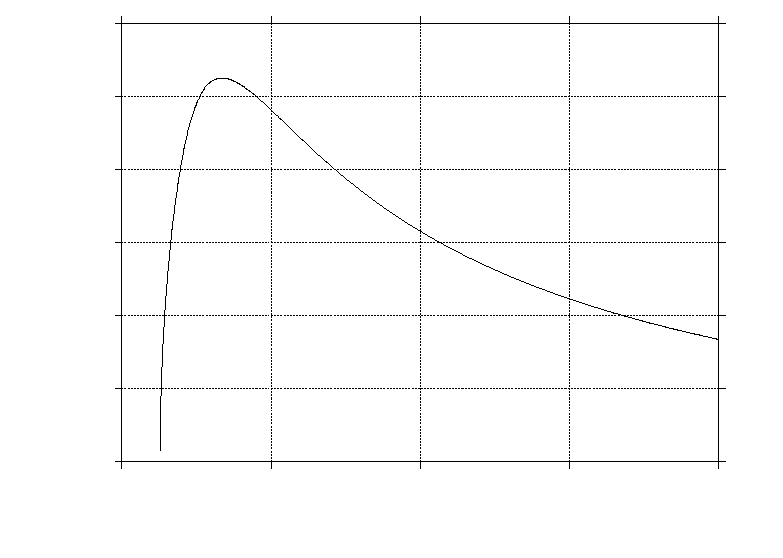
\includegraphics{Figures/twowires/Deltas3.1.3/nBdepend}}%
    \gplfronttext
  \end{picture}%
\endgroup
  
\caption{Solid line: the critical distance $d_c$ plotted as a function of the ratio of interparticle distances $n_F/n_B^{1/3}$. White background: intrawire pairing only regime. Grey background: interwire pairing only regime. Dash-dotted line: the critical distance according to the competition of intra- and interwire interactions for $k_Fx_0 = 1/\sqrt{3}$. See equation \eqref{eq.2wires.Vequal}. When we cross the solid line the system experiences the phase transition studied in section \ref{sec.2wiresCrossover_energy}. Dashed vertical line: $v_F = c_0$. The curve to the right hereof is only the zero frequency contribution. Parameters: $(n_Ba_B^3)^{1/3} = 0.01$, $(n_Ba_{BF}^3)^{1/3} = 0.11$, $l_t = 0$, $\frac{m_B}{m_F} = 7/40$. }  
\label{fig.twowirescrossovernBdepend}  
\end{center}    
\end{figure}

In this way we explicitly see, that instead of actually moving the wires we can control the cross over by adjusting $n_F/n_B^{1/3}$ and in turn the coherence length; see equation \eqref{eq.RangefunctionofrBBnB}. This all supports the intuitive idea outlined above. Caution should however be taken. Most importantly, there is an extremal value of $d_c$ at a finite value of $n_F/n_B^{1/3}$. Notice, that this also means, that just below this extremal value, there is an interval of distances, where the system experiences two cross overs. This is not explained by the competition of interactions. This we can see quite explicitly by solving equation \eqref{eq.2wires.Vequal} numerically. However, we have to choose a specific value of $x_0$. In the $\xi \to \infty$ limit we get a solvable form of the equation:
\begin{equation}
2 = \sqrt{1 + \left(\frac{d_c}{x_0}\right)^2} \Rightarrow d_c = \sqrt{3} x_0. \nonumber
\end{equation}
From this it is clear, that $d_c$ reaches a constant for $\xi \to \infty$ based on \eqref{eq.2wires.Vequal}. Hence, the fact that the actual critical distance $d_c$ has this asymptotic behaviour is well-described within a competition of interactions line of thinking. Further, in this line of thinking it is physically reasonable, that the asymptotic value of $d_c$ is the typical distance between the particles: $k_Fd_c = 1$.\footnote{This choice is reasonable, but not crucial. For any value of $x_0 > 0$ the result is the same.} Hence, we set $k_Fx_0 = 1/\sqrt{3}$. This results in the dash-dotted line in figure \ref{fig.twowirescrossovernBdepend}. From this it is clear, that the competition of interactions is not able to capture the fact, that the dependence of the critical distance, $d_c$, on the ratio of interparticle distances, $n_F/n_B^{1/3}$, is \textit{not} monotonic, but rather has a maximal value at a finite value of $n_F/n_B^{1/3}$ as mentioned above. This emphasizes the fact, that although a lot of physical intuition can be build on the form and behaviour of the interactions, we have to be careful when using it to argue for the response of the system.

Let us try to understand this from a functional point of view instead. The intrawire pairing, $\Delta^{11}_k$, depends on the parameters $\beta, m_B/m_F, (n_Ba_B^3)^{1/3}$ and $n_B^{1/3}/n_F$ and is a functional of the pairings themselves: $\Delta^{11}_k, \Delta^{12}_k$. This is similarly the case for the interwire pairing, $\Delta^{12}_k$, with the additional parameter $d$. Hence, we can write:
\begin{equation}
\Delta^{11}_k = G\left(\Delta^{11}_k, \Delta^{12}_k, \beta, \frac{m_B}{m_F}, (n_Ba_B^3)^{1/3}, \frac{n_B^{1/3}}{n_F} \right), \hspace{0.5cm} \Delta^{12}_k = H\left(\Delta^{11}_k, \Delta^{12}_k, \beta, \frac{m_B}{m_F}, (n_Ba_B^3)^{1/3}, \frac{n_B^{1/3}}{n_F}, d \right), \nonumber 
\end{equation}
where $G$ and $H$ are the described functionals. On unitless form the functionals have a common prefactor, that depends on the mass ratio, the Bose gas parameter and the ratio of interparticle distances: $m_B/m_F, (n_Ba_B^3)^{1/3}$, and $n_B^{1/3}/n_F$. This means, that the limit of $n_F/n_B^{1/3} \to \infty $ is well-defined for the ratio of the pairings:
\begin{equation}
\lim_{\frac{n_F}{n_B^{1/3}} \to \infty} \left[\frac{|\Delta^{11}_{k_F}|]}{|\Delta^{12}_{k_F}|}\right] = \frac{\left|G\left(\Delta^{11}_{k_F}, \Delta^{12}_{k_F}, \beta, \frac{m_B}{m_F}, (n_Ba_B^3)^{1/3}, \frac{n_B^{1/3}}{n_F} = 0 \right)\right|}{\left|H\left(\Delta^{11}_{k_F}, \Delta^{12}_{k_F}, \beta, \frac{m_B}{m_F}, (n_Ba_B^3)^{1/3}, \frac{n_B^{1/3}}{n_F} = 0, d \right)\right|}. \nonumber
\end{equation}
Since the pairings at $k_F$ must be comparable at a distance similar to $d_c$, the above ratio will be equal to 1 at a distance similar to $d_c$. It is therefore evident that $d_c$ is independent of the ratio of interparticle distances for $n_F/n_B^{1/3} \gg 1$. Hence, $d_c$ must approach a constant for increasing values of $n_F/n_B^{1/3}$. 

The appearance of a maximum in $d_c$ can qualitatively be understood in the following way. For low values of $n_F/n_B^{1/3}$ the Bose gas becomes more rigid, since the spacing between the bosons becomes smaller. Hence, the wires must be brought closer together for the interwire pairing to dominate. For high values of $n_F/n_B^{1/3}$ the Bose gas is depleted. This means, that there are simply fewer bosons for the fermions to interact with. It is therefore reasonable, that $d_c$ should not exhibit a maximal value for $n_F/n_B^{1/3} \to \infty$. As a consequence a maximal value of $d_c$ appeares. This analysis is reminiscent of the analysis explaning the appearance of a minimum in intrawire effective interaction, $W_\text{ind}^{11}(k_F,k_F)$, as a function of $n_F/n_B^{1/3}$. See subsection \ref{subsec.relevantmomenta.effectiveinteraction} for the details.  

\section{Temperature dependency of pairings}
In this section we will investigate, how the pairings depend on temperature. The analysis is performed in complete analogy to the one in subsection \ref{subsec.momentum_and_temperature_pairing_singlewire}. 

For small and large distances, where one of the pairings is dominant, it is not difficult to imagine, what will happen. Here we expect, that the two pairings go to zero in a similar manner to single wire at two different critical temperatures. The dominant pairing for $T = 0$ will have the highest critical temperature. However, a couple questions arise. How does it affect the dominant pairing, that the suppressed pairing goes to zero? And is the interwire or intrawire pairing the more robust to a rise in temperature?

To answer these questions we investigate three cases, two where one pairing is strongly dominant, and one where the pairings are essentially equal for $T = 0$. The more interesting case is definitely the latter one, since this directly tests what pairing is the more robust. However, we might also gain some insight from the former. 

The result of the analysis for a dominant interwire pairing is shown in figure \ref{fig.maximalpairingsTdepend_2wires}. We see, that the overall expected behaviour is observed. We observe that the intrawire pairing has a small downward kink, where the interwire pairing vanishes. The same behaviour is seen when the interwire pairing is dominant. This has to implications. The first is, that the dominant pairing would be higher at low temperatures if the other pairing was not present: there is a trade off between the size of the individual pairings and the presence of a second pairing. The second is, that the presence of a second smaller pairing seem to stabilize the dominant one, since the kink is downwards for increasing temperatures. Further, above the critical temperature of the smaller pairing, the maximal intrawire pairing of the dominating pairing is well described by the following relation:
\begin{equation}
\max_k[\Delta^{\text{dom}}_k(T)] = \alpha \max_k[\Delta^{\text{dom}}_k(T = 0)] \sqrt{1 - \left(\frac{T}{T_c}\right)^3},
\label{eq.DeltaapproxaboveTC1}
\end{equation}
where $\text{dom}$ is short for dominating. This has the same form as the approximate form in equation \eqref{eq.maxpairingapprox} apart from the $\alpha$. The coefficient $\alpha$ is slightly bigger than $1$, but seems to depend slightly on the other parameters of the problem. For the present set of parameters we have $\alpha = 1.3$. 

\begin{figure} 
\begin{center}  
% GNUPLOT: LaTeX picture with Postscript
\begingroup
  \makeatletter
  \providecommand\color[2][]{%
    \GenericError{(gnuplot) \space\space\space\@spaces}{%
      Package color not loaded in conjunction with
      terminal option `colourtext'%
    }{See the gnuplot documentation for explanation.%
    }{Either use 'blacktext' in gnuplot or load the package
      color.sty in LaTeX.}%
    \renewcommand\color[2][]{}%
  }%
  \providecommand\includegraphics[2][]{%
    \GenericError{(gnuplot) \space\space\space\@spaces}{%
      Package graphicx or graphics not loaded%
    }{See the gnuplot documentation for explanation.%
    }{The gnuplot epslatex terminal needs graphicx.sty or graphics.sty.}%
    \renewcommand\includegraphics[2][]{}%
  }%
  \providecommand\rotatebox[2]{#2}%
  \@ifundefined{ifGPcolor}{%
    \newif\ifGPcolor
    \GPcolorfalse
  }{}%
  \@ifundefined{ifGPblacktext}{%
    \newif\ifGPblacktext
    \GPblacktexttrue
  }{}%
  % define a \g@addto@macro without @ in the name:
  \let\gplgaddtomacro\g@addto@macro
  % define empty templates for all commands taking text:
  \gdef\gplbacktext{}%
  \gdef\gplfronttext{}%
  \makeatother
  \ifGPblacktext
    % no textcolor at all
    \def\colorrgb#1{}%
    \def\colorgray#1{}%
  \else
    % gray or color?
    \ifGPcolor
      \def\colorrgb#1{\color[rgb]{#1}}%
      \def\colorgray#1{\color[gray]{#1}}%
      \expandafter\def\csname LTw\endcsname{\color{white}}%
      \expandafter\def\csname LTb\endcsname{\color{black}}%
      \expandafter\def\csname LTa\endcsname{\color{black}}%
      \expandafter\def\csname LT0\endcsname{\color[rgb]{1,0,0}}%
      \expandafter\def\csname LT1\endcsname{\color[rgb]{0,1,0}}%
      \expandafter\def\csname LT2\endcsname{\color[rgb]{0,0,1}}%
      \expandafter\def\csname LT3\endcsname{\color[rgb]{1,0,1}}%
      \expandafter\def\csname LT4\endcsname{\color[rgb]{0,1,1}}%
      \expandafter\def\csname LT5\endcsname{\color[rgb]{1,1,0}}%
      \expandafter\def\csname LT6\endcsname{\color[rgb]{0,0,0}}%
      \expandafter\def\csname LT7\endcsname{\color[rgb]{1,0.3,0}}%
      \expandafter\def\csname LT8\endcsname{\color[rgb]{0.5,0.5,0.5}}%
    \else
      % gray
      \def\colorrgb#1{\color{black}}%
      \def\colorgray#1{\color[gray]{#1}}%
      \expandafter\def\csname LTw\endcsname{\color{white}}%
      \expandafter\def\csname LTb\endcsname{\color{black}}%
      \expandafter\def\csname LTa\endcsname{\color{black}}%
      \expandafter\def\csname LT0\endcsname{\color{black}}%
      \expandafter\def\csname LT1\endcsname{\color{black}}%
      \expandafter\def\csname LT2\endcsname{\color{black}}%
      \expandafter\def\csname LT3\endcsname{\color{black}}%
      \expandafter\def\csname LT4\endcsname{\color{black}}%
      \expandafter\def\csname LT5\endcsname{\color{black}}%
      \expandafter\def\csname LT6\endcsname{\color{black}}%
      \expandafter\def\csname LT7\endcsname{\color{black}}%
      \expandafter\def\csname LT8\endcsname{\color{black}}%
    \fi
  \fi
    \setlength{\unitlength}{0.0500bp}%
    \ifx\gptboxheight\undefined%
      \newlength{\gptboxheight}%
      \newlength{\gptboxwidth}%
      \newsavebox{\gptboxtext}%
    \fi%
    \setlength{\fboxrule}{0.5pt}%
    \setlength{\fboxsep}{1pt}%
\begin{picture}(7200.00,5040.00)%
    \gplgaddtomacro\gplbacktext{%
      \csname LTb\endcsname%
      \put(814,767){\makebox(0,0)[r]{\strut{}$0$}}%
      \csname LTb\endcsname%
      \put(814,1609){\makebox(0,0)[r]{\strut{}$0.1$}}%
      \csname LTb\endcsname%
      \put(814,2451){\makebox(0,0)[r]{\strut{}$0.2$}}%
      \csname LTb\endcsname%
      \put(814,3292){\makebox(0,0)[r]{\strut{}$0.3$}}%
      \csname LTb\endcsname%
      \put(814,4134){\makebox(0,0)[r]{\strut{}$0.4$}}%
      \csname LTb\endcsname%
      \put(814,4976){\makebox(0,0)[r]{\strut{}$0.5$}}%
      \csname LTb\endcsname%
      \put(1009,484){\makebox(0,0){\strut{}$0$}}%
      \csname LTb\endcsname%
      \put(1964,484){\makebox(0,0){\strut{}$0.05$}}%
      \csname LTb\endcsname%
      \put(2919,484){\makebox(0,0){\strut{}$0.1$}}%
      \csname LTb\endcsname%
      \put(3875,484){\makebox(0,0){\strut{}$0.15$}}%
      \csname LTb\endcsname%
      \put(4830,484){\makebox(0,0){\strut{}$0.2$}}%
      \csname LTb\endcsname%
      \put(5785,484){\makebox(0,0){\strut{}$0.25$}}%
      \csname LTb\endcsname%
      \put(6740,484){\makebox(0,0){\strut{}$0.3$}}%
    }%
    \gplgaddtomacro\gplfronttext{%
      \csname LTb\endcsname%
      \put(176,2871){\rotatebox{-270}{\makebox(0,0){\strut{}$\max_k[\Delta_k]/\epsilon_{F,0}$}}}%
      \put(3874,154){\makebox(0,0){\strut{}$T/T_F$}}%
    }%
    \gplbacktext
    \put(0,0){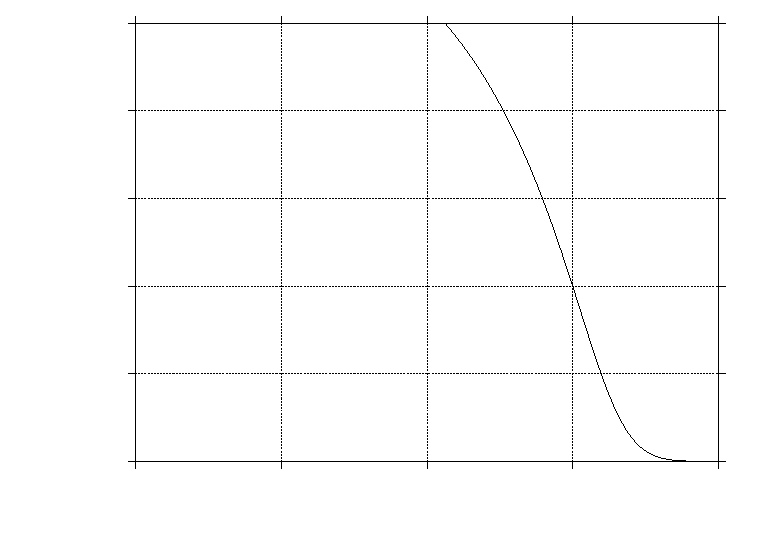
\includegraphics{Figures/twowires/Deltas4.5/Tdepend}}%
    \gplfronttext
  \end{picture}%
\endgroup
  
\caption{Blue solid line: $\max_k[|\Delta^{12}_k|]$ as a function of temperature. Blue dashed line: approximate form from the single wire analysis, equation \eqref{eq.maxpairingapprox}. Red solid line: $\max_k[|\Delta^{11}_k|]$ as a function of temperature. Red dashed line: Approximate form according to equation \eqref{eq.DeltaapproxaboveTC1} above the critical temperature of the interwire pairing. Notice, that there are two critical temperatures, and that the intrawire pairing shows a downward kink, where the interwire pairing goes to zero. Parameters: $k_Fd = 0.61$, $(n_Ba_B^3)^{1/3} = 0.01$, $(n_Ba_{BF}^3)^{1/3} = 0.11$, $l_t = 0$, $\frac{m_B}{m_F} = 7/40$, $\frac{n_F}{n_B^{1/3}} = 0.215$, $v_F/c_0 = 0.33$.}  
\label{fig.maximalpairingsTdepend_2wires}  
\end{center}    
\end{figure} 



 


